\subsection{Regiões de credibilidade}

Na Seção passada estudamos 
o problema de estimação,
em que desejamos escolher 
um número próximo ao parâmetro.
Como resposta, obtivemos que 
medidas de centralidade da distribuição a posteriori
são obtidas como estimadores ótimos.
Por exemplo, a média a posteriori é 
o estimador ótimo para a utilidade quadrática e
a mediana a posteriori é o estimador ótimo para
a utilidade obtida pelo desvio absoluto.
Pelo fato de a resposta para 
um problema de estimação ser um único número,
ela não indica o quanto temos certeza de que
o parâmetro está próximo desse número.

Nesta Seção, estudaremos o problema de decisão que
consiste em obter regiões de credibilidade.
Em outras palavras, o problema de obter 
um subconjunto do espaço paramétrico no qual 
o parâmetro provavelmente está contido.
Contudo, também desejamos que o intervalo seja 
o menor possível, para que tenhamos mais 
precisão a respeito de qual é o valor do parâmetro.
Assim como no problema de estimação, 
existem várias funções de perda que
buscam capturar estas idéias. 
A seguir, estudaremos algumas destas funções.

\subsubsection{Intervalos de credibilidade}

Iniciaremos a análise buscando intervalos que 
provavelmente contém o parâmetro.
Um intervalo é definido como $[a,b]$, 
onde $a \in \mathbb{R}$, $b \in \mathbb{R}$ e 
$a \leq b$. Assim, o conjunto de alternativas simples é $\mathcal{A}_{*} = \{(a,b) \in \mathbb{R}^{2}: a \leq b\}$.

Uma possível função de utilidade para 
este problema é dada por
\begin{align*}
 U((a,b),\theta)
 &= \I(\theta \in [a,b]) -k(b-a)
 & k > 0
\end{align*}
O elemento $\I(\theta \in [a,b])$ indica que 
é desejável que $\theta$ esteja no intervalo.
O elemento $-k(b-a)$ indica que 
é desejável que o intervalo seja pequeno.
\begin{theorem}
 \label{thm:credible_interval_1}
 Se $U((a,b),\theta) = \I(\theta \in [a,b]) -k(b-a)$,
 então a decisão ótima, $(a^{*}(X),b^{*}(X))$ satisfaz
 \begin{align*}
  f_{\theta|X}(a^{*}|X)
  =f_{\theta|X}(b^{*}|X) = k
 \end{align*}
\end{theorem}
\begin{proof}
 Podemos deduzir o intervalo ótimo neste caso 
 usando o \cref{theorem:extensive-form}. 
 \begin{align*}
  \E[U((a,b),\theta)|X]	
  &= \E[\I(\theta \in [a,b]) -k(b-a)|X] \\
  &= \P(\theta \in [a,b]|X) -k(b-a) \\
  &= \int_{a}^{b}{f(\theta|X)d\theta} -k(b-a) \\
  &= \left(ka-\int_{-\infty}^{a}{f(\theta|X)d\theta}\right) 
  +\left(\int_{-\infty}^{b}{f(\theta|X)d\theta}-kb\right)
 \end{align*}
 Portanto, temos que
 \begin{align*}
  \nabla \E[U((a,b),\theta)|X]
  &= (k-f_{\theta|X}(a|X), f_{\theta|X}(b|X)-k)
 \end{align*}
\end{proof}
Assim, para que $(a,b)$ seja um ponto de máximo,
é necessário que
$f_{\theta|X}(a|X) = f_{\theta|X}(b|X) = k$.
Em geral, podem existir vários pontos que 
satisfazem esta propriedade.
Neste caso, devemos testar 
todas as possíveis combinações de pontos
e escolher aquela que maximiza a utilidade esperada.
Em particular, se $f_{\theta|X}(\cdot|X)$ é unimodal, 
então apenas existem dois pontos 
$(a,b) \in \mathbb{R}^{2}$ tais que 
$f_{\theta|X}(a|X) = f_{\theta|X}(b|X) = k$ e temos que
$[a,b] = \{\theta: f(\theta|X) \geq k\}$.
Note que é possível tomar $k$ de tal forma que 
$\P(\theta \in [a,b]|X) = 1-\alpha$.
Neste caso, dizemos que construímos um 
intervalo de credibilidade com 
credibilidade $1-\alpha$ (veja Seção \ref{sec:credibilidade}).

Outra possível função utilidade é
\begin{align*}
 U((a,b),\theta)
 &= -k_{1}((a-\theta)_{+} +(\theta-b)_{+}) -k_{2}(b-a)
 & \text{, onde } (x-y)_{+} = \max(0,x-y) \\
 && k_{1},k_{2} > 0
\end{align*}
Similarmente à utilidade anterior, 
o elemento $-k_{2}(b-a)$ indica que 
é desejável que o intervalo seja pequeno.
Como contraponto, o elemento 
$-k_{1}((a-\theta)_{+} + (\theta-b)_{+}) -k_{2}(b-a)$
indica que é desejável que 
a distância de $\theta$ a $[a,b]$ seja baixa e,
em particular, que $\theta$ esteja dentro de $[a,b]$.
\begin{theorem}
 \label{thm:credible_interval_2}
 Se $U((a,b),\theta) =-k_{1}((a-\theta)_{+} + (\theta-b)_{+}) -k_{2}(b-a)$, então
 a melhor decisão $(a,b)$ é tal que 
 $a$ e $b$ são, respectivamente, o 
 $\frac{k_{2}}{k_{1}}$-ésimo
 e $1-\frac{k_2}{k_1}$-ésimo 
 percentis da \emph{posteriori} para $\theta$ dado $X$.
\end{theorem}
\begin{proof}
 Podemos deduzir o intervalo ótimo neste caso
 usando o \cref{theorem:extensive-form}. 
 \begin{align*}
  \E[U((a,b),\theta)|X]	
  &= \E[-k_{1}((a-\theta)_{+} +(\theta-b)_{+}) 
  -k_{2}(b-a)|X] \\
  &= -k_{1}(\E[(a-\theta)_{+}|X]+\E[(\theta-b)_{+}|X]) 
  -k_{2}(b-a) \\
  &= -k_{1}\left(\int_{-\infty}^{a}{(a-\theta)f(\theta|X)d\theta}
  +\int_{b}^{\infty}{(\theta-b)f(\theta|X)d\theta}\right)
  -k_{2}(b-a) \\
  &=  \underbrace{\left(-k_{1}\int_{-\infty}^{a}{(a-\theta)f(\theta|X)d\theta}+k_{2}a\right)}_{g(a)} + \underbrace{\left(-k_{1}\int_{b}^{\infty}{(\theta-b)f(\theta|X)d\theta}-k_{2}b\right)}_{h(b)}
 \end{align*}
 Portanto, podemos tomar $a$ maximizando $g(a)$ e
 $b$ maximizando $h(b)$.
 Note que
 \begin{align*}
  g(a)	
  &= -k_{1}\int_{-\infty}^{a}{(a-\theta)f(\theta|X)d\theta}+k_{2}a \\
  &= -k_{1}a\int_{-\infty}^{a}{f(\theta|X)d\theta}+k_{1}\int_{-\infty}^{a}{\theta f(\theta|X)d\theta}+k_{2}a
 \end{align*}
 Portanto, pelo Teorema Fundamental do Cálculo,
 \begin{align*}
  g'(a)	&= -k_{1}\int_{-\infty}^{a}{f(\theta|X)d\theta} -k_{1}af(a|X) +k_{1}af(a|X) + k_{2} \\
  &= -k_{1}\int_{-\infty}^{a}{f(\theta|X)d\theta} + k_{2}
 \end{align*}
 Assim, para que $g'(a) = 0$, é necessário que
 \begin{align*}
  \int_{-\infty}^{a}{f(\theta|X)d\theta}
  &= \frac{k_{2}}{k_{1}} \\
  \P(\theta \leq a|X)
  &= \frac{k_{2}}{k_{1}}
 \end{align*}
 Ou seja, $a$ deve ser o 
 $\frac{k_2}{k_1}$-ésimo percentil da 
 \emph{posteriori} para $\theta$ dado $X$.
 Similarmente, para $b$, obtemos 
 \begin{align*}
  h(b)	
  &= -k_{1}\int_{b}^{\infty}
  {(\theta-b)f(\theta|X)d\theta}-k_{2}b	\\
  &= -k_{1}\int_{b}^{\infty}{\theta f(\theta|X)d\theta}
  +k_{1}b\int_{b}^{\infty}{f(\theta|X)d\theta} -k_{2}
 \end{align*}
 Portanto, pelo Teorema Fundamental do Cálculo,
 \begin{align*}
  h'(b)	&= k_{1}bf(b|X)+k_{1}\int_{b}^{\infty}{f(\theta|X)d\theta}-k_{1}bf(b|X) - k_{2}b \\
  &= k_{1}\int_{b}^{\infty}{f(\theta|X)d\theta} -k_{2}
 \end{align*}
 Assim, para que $h'(b) = 0$, é necessário que
 \begin{align*}
  \int_{b}^{\infty}{f(\theta|X)d\theta}
  &= \frac{k_2}{k_1} \\
  \P(\theta \geq b|X)
  &= \frac{k_2}{k_1} \\
  \P(\theta < b|X)										
  &= 1-\frac{k_2}{k_1}
 \end{align*}
 Ou seja, $b$ deve ser o 
 $1-\frac{k_2}{k_1}$-ésimo percentil da 
 \emph{posteriori} para $\theta$ dado $X$.
\end{proof}
Note que apenas os valores relativos entre
$k_1$ e $k_2$ são relevantes para a decisão tomada.
Por exemplo, o mesmo intervalo será obtido se 
$k_1=1$ e $k_2=0.5$ ou se $k_1=2$ e $k_2=1$.
Também note que é possível tomar $k_1$ e $k_2$ 
de tal forma que $\P(\theta \in [a,b]|X) = 1-\alpha$.
Para tal, basta escolher 
$\frac{k_2}{k_1} = \frac{\alpha}{2}$ 
Neste caso, dizemos que construímos um intervalo de credibilidade com credibilidade $1-\alpha$.

O último intervalo de credibilidade que 
veremos é baseado na utilidade
\begin{align*}
 U((a,b),\theta)
 &= -k_{1}(b-a)
 -\frac{k_{2}}{b-a}\left(\theta -\frac{a+b}{2}\right)^{2}
 & k_{1},k_{2} > 0
\end{align*}
Similarmente às utilidades anteriores,
$-k_{1}(b-a)$ indica que 
é desejável que o intevalo seja pequeno.
Também, $\frac{a+b}{2}$ é o centro do intervalo.
Assim, $-\frac{k_{2}}{b-a}\left(\theta - \frac{a+b}{2}\right)^{2}$ indica que 
é desejável que o centro do intervalo esteja
próximo a $\theta$.
\begin{theorem}
 \label{thm:credible_interval_3}
 Se $U((a,b),\theta) = -k_{1}(b-a) -\frac{k_{2}}{b-a}\left(\theta - \frac{a+b}{2}\right)^{2}$,
 então a melhor alternativa é tal que
 \begin{align*}
  [a,b]	&= \left[E[\theta|X]-2^{-1}\sqrt{\frac{k_2}{k_1}Var[\theta|X]}, E[\theta|X]+2^{-1}\sqrt{\frac{k_2}{k_1}Var[\theta|X]}\right]
 \end{align*}
\end{theorem}
\begin{proof}
 Podemos deduzir o intervalo ótimo neste caso 
 usando o \cref{theorem:extensive-form}.
 \begin{align}
  \label{eq:ic_1}
  \E[U((a,b),\theta)|X]	
  &= \E\left[-k_{1}(b-a)-\frac{k_{2}}{b-a}\left(\theta - \frac{a+b}{2}\right)^{2}|X\right]	\nonumber \\
  &= -k_{1}(b-a) -\frac{k_{2}}{b-a}\E\left[\left(\theta - \frac{a+b}{2}\right)^{2}|X\right]	\nonumber \\
  &= -k_{1}t -\frac{k_{2}}{t}\E\left[(\theta-c)^{2}|X\right]
  & t=b-a, c=\frac{a+b}{2} \nonumber \\
  &= -k_{1}t -\frac{k_{2}}{t}\left(\V[\theta|X]
  +(\E[\theta|X]-c)^{2}\right)
  & \text{\cref{lemma:conditional_l2}}
 \end{align}
 Note que, qualquer que seja o valor de $t$, 
 a expressão em \cref{eq:ic_1} é maximizada 
 tomando $c^{*}=E[\theta|X]$.
 Substituindo esse valor em \cref{eq:ic_1}, obtemos
 \begin{align*}
  \E[U((a,b),\theta)|X]	
  &= -k_{1}t -\frac{k_{2}}{t}\V[\theta|X]
 \end{align*}
 Para achar o ponto de máximo dessa expressão, 
 determinamos o seu ponto crítico
 \begin{align*}
  \frac{d\E[U((a,b),\theta)|X]}{dt}	
  &= -k_{1} +k_{2}t^{-2}\V[\theta|X]
 \end{align*}
 Assim, $\frac{d\E[U((a,b),\theta)|X]}{dt}=0$ para 
 $t^{*} = \sqrt{\frac{k_2}{k_1}\V[\theta|X]}$.
 Como
 \begin{align*}
  \frac{d^{2}\E[U((a,b),\theta)|X]}{dt^{2}} 
  &= -2k_{2}t^{-3}\V[\theta|X] < 0
 \end{align*}
 $t^{*}$ é um ponto de máximo de 
 $\E[U((a,b),\theta)|X]$.
 O resultado final é obtido usando 
 $c^{*}=\frac{a+b}{2}$ e $t^{*}=b-a$.
\end{proof}

\subsubsection{Regiões de credibilidade}

Na subseção anterior utilizamos 
intervalos para resumir a informação a respeito 
da distribuição a posteriori.
Em geral, construímos os intervalos de credibilidade
de tal forma que eles fossem pequenos e 
contivessem o parâmetro com alta probabilidade.
Contudo, em algumas ocasiões, 
um intervalo pode ser inadequado para obter estes objetivos.
Por exemplo, considere que
\begin{align*}
 f(\theta|X)
 &= \frac{1}{2\sqrt{2\pi}}\exp(-\theta^{2})
 +\frac{1}{2\sqrt{2\pi}}\exp(-(\theta^{2}-100))
\end{align*}
Esta é a distribuição obtida misturando-se 
duas normais com  variâncias iguais a $1$ e 
médias iguais a $0$ e $100$.
A densidade $f(\theta|X)$ é apresentada na
\cref{figure:normal-mixture-1}.
Note que $\E[\theta|X] = 50$.
Assim, se usarmos a terceira 
função de utilidade da subseção passada,
o intervalo de credibilidade obtido será
da forma $[50-k,50+k]$.
Usando um software computacional,
encontramos que $k=51.7$ gera 
um intervalo de credibilidade próxima a 95\%.
Contudo, o intervalo obtido, $[-1.7,101.7]$, 
não resume adequadamente $f(\theta|X)$.
Isso ocorre pois o intervalo inclui 
os valores de baixa densidade próximos a $50$.
\begin{figure}
 \centering
 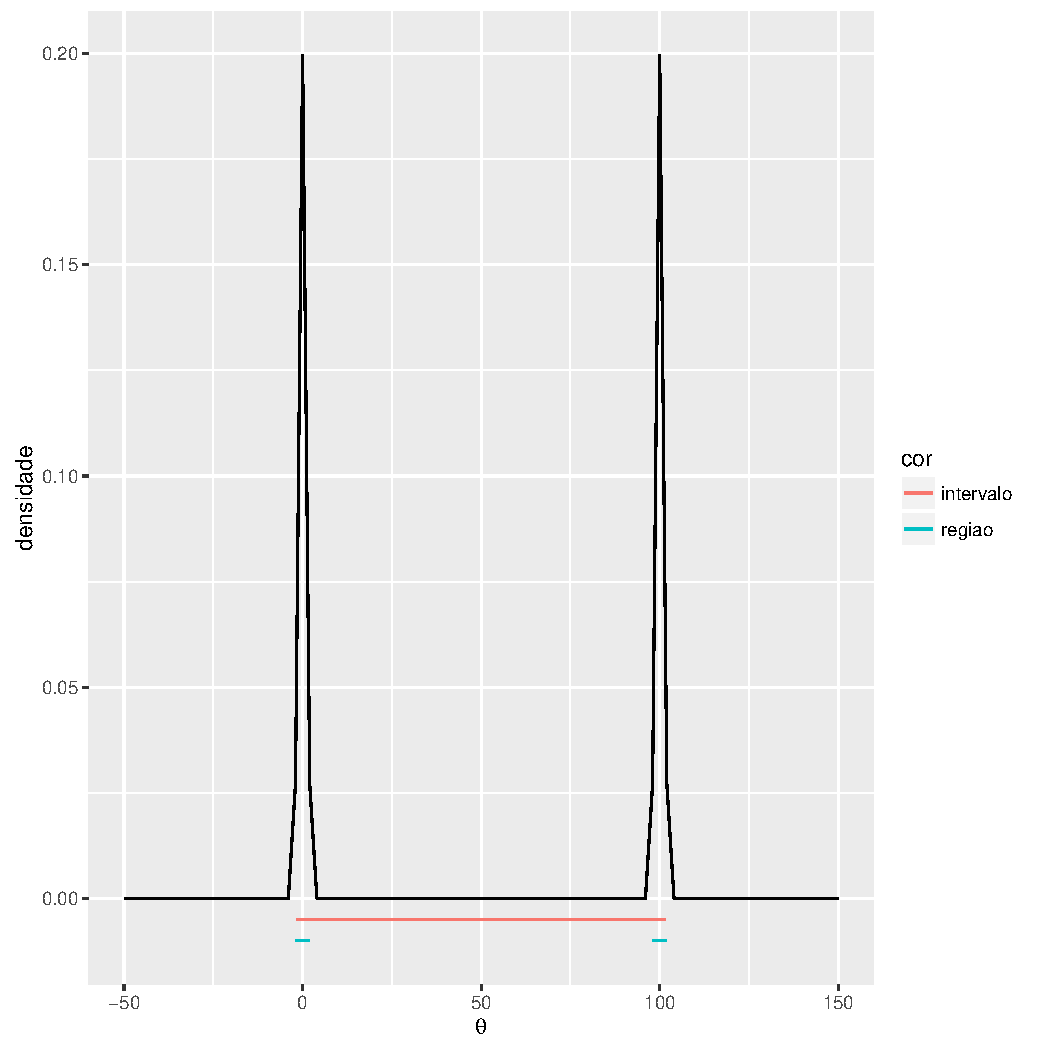
\includegraphics[scale=0.5]{chapter-decisions-normal-mixture.pdf}
 \caption{Densidade da mistura de 
 uma $N(0,1)$ e uma $N(100,1)$
 acompanhada de um intervalo de credibilidade e
 de uma região de credibilidade.}
 \label{figure:normal-mixture-1}
\end{figure}

Como uma alternativa a um 
intervalo de credibilidade,
poderíamos combinar um 
intervalo de credibilidade para cada 
uma das normais na mistura.
Sabemos que uma $N(0,1)$ tem 
probabilidade de $95\%$ de estar em $[-1.96,1.96]$.
Similarmente, a $N(100,1)$ tem 
probabilidade de $95\%$ de estar em $[98.04,101.96]$.
Assim, a mistura de 
uma $N(0,1)$ e uma $N(100,1)$ tem 
alta probabilidade de estar em 
$[-1.96,1.96] \cup [98.04,101.96]$.
Neste exemplo, intervalos são 
demasiadamente restritivos e 
não descrevem adequadamente 
a \emph{posteriori} multimodal.

Assim, nesta subseção consideraremos 
um problema de decisão em que,
ao invés de escolher um intervalo para 
descrever a posteriori,
é necessário escolher uma região para fazê-lo.
De forma geral, uma região pode ser 
qualquer subconjunto do espaço paramétrico.
Assim, temos que
$\mathcal{A}_{*} = \{R \subset \Theta\}$.
Para estudar este problema de decisão,
consideraremos a seguinte função de utilidade
\begin{align*}
 U(R(X),\theta)	
 &= \I(\theta \in R(X)) 
 -k\int_{x \in R(x)}{1 \cdot dx}
 & k > 0
\end{align*}
O elemento $\I(\theta \in R(X))$ indica que 
é desejável que $\theta$ esteja 
na região de credibilidade, $R(X)$.
Por outro lado,  $\int_{x \in R(x)}{dx}$ indica que
é desejável que a região $R(x)$ seja pequena, 
ou seja, tenha um volume pequeno.
\begin{theorem}
 \label{thm:hpd}
 Se $U(R(X),\theta)	= \I(\theta \in R(X)) - k\int_{x \in R(x)}{1 \cdot dx}$, então 
 a melhor região de credibilidade é tal que 
 $R(X) = \{\theta \in \Theta: f(\theta|X) \geq k\}$.
 Dizemos que $R(X)$ é um HPD (highest posterior density) 
 de $f(\theta|X)$.
\end{theorem}


\subsubsection{Regiões de credibilidade com credibilidade especificada}
 \label{sec:credibilidade}
 
 
Na prática, é comum criar uma região de credibilidade
de modo que a probabilidade (a posteriori) do parâmetro estar nessa região
seja um valor pré-especificado $1-\alpha$. Este valor de cobertura é chamado de 
\emph{credibilidade} dessa região:
\begin{definition}
Dizemos que uma região $R \subset \Theta$ tem credibilidade $1-\alpha$
se $\P(\theta \in R|\x)=1-\alpha$.
\end{definition}

Assim, é comum escolher o formato da região desejada usando 
alguma das funções de perda apresentadas nesta seção, e então buscar, dentre essas regiões,
aquela que tem a credibilidade desejada.

\begin{example}
Considere novamente o Exemplo \ref{exemplo:eleicao}.
Vamos construir intervalos de credibilidade
para $\theta$.
Para tanto, lembre-se que $\theta|X=20 \sim \mbox{Beta}(25,15)$.
O seguinte código ilustra como encontrar os intervalos de credibilidade
investigados nesta seção, com constantes na utilidade escolhidas de modo que a credibilidade dos intervalos seja $95\%$.


\begin{knitrout}
\definecolor{shadecolor}{rgb}{0.969, 0.969, 0.969}\color{fgcolor}\begin{kframe}
\begin{alltt}
\hlstd{a} \hlkwb{<-} \hlnum{25} \hlcom{# parâmetros a posteriori}
\hlstd{b} \hlkwb{<-} \hlnum{15} \hlcom{# posteriori}
\end{alltt}
\end{kframe}
\end{knitrout}


\end{example}

\subsubsection*{Exercícios}

\begin{exercise}
 \label{ex:normal-credible}
 Dado $\mu$, $X_{1},\ldots,X_{n}$ são i.i.d. e 
 $X_{1} \sim N(\mu,1)$.
 \emph{A priori}, $\mu \sim N(0,1)$.
 \begin{enumerate}[label=(\alph*)]
  \item Ache um estimador para $\mu$ usando 
  cada utilidade que vimos em aula.
  \item Ache um intervalo para $\mu$ com 
  credibilidade $95\%$ para 
  cada utilidade que vimos em aula.
  \item Ache o HPD para $\mu$.
 \end{enumerate}
\end{exercise}

\solution{\textbf{Solução}:
 Decorre do \cref{ex:conjugate-normal-normal} que
 $\theta|X \sim N(\frac{n\bar{X}}{n+1},n+1)$.
 \begin{enumerate}[label=(\alph*)]
  \item Sabemos que, para a distância quadrática
  (\cref{thm:estimation_l2}), 
  o estimador ótimo é $E[\theta|X]$ e,
  para a distância em valor absoluto
  (\cref{thm:estimation_l1}), ele é $Med[\theta|X]$.
  Como a distribuição normal é 
  simétrica em torno da média, temos que 
  $Med[\theta|X] = E[\theta|X] = \frac{n\bar{X}}{n+1}$.
  
  \item \begin{itemize}
   \item Como a distribuição normal é unimodal,
   o intervalo de credibilidade pelo
   \cref{thm:credible_interval_1} é da forma 
   \begin{align*}
    [a,b] = \{\theta \in \Theta: f(\theta|X) \geq k\}
   \end{align*}
   Também, como a distribuição normal é 
   simétrica em torno de $\E[\theta|X]$ e unimodal,
   existe $c$ tal que
   \begin{align*}
    \{\theta \in \Theta: f(\theta|X) \geq k\} 
    &= [\E[\theta|X]-c,\E[\theta|X]+c]
   \end{align*}
   Assim, desejamos achar $c$ tal que
   \begin{align*}
    \P(\theta \in [\E[\theta|X]-c,\E[\theta|X]+c]|X)
    &= 95\%	\\
    \P\left(\frac{\theta
    -\E[\theta|X]}{\sqrt{\V[\theta|X]}} 
    \in \left[-\frac{c}{\sqrt{\V[\theta|X]}},
    \frac{c}{\sqrt{\V[\theta|X]}}\right]|X\right)	
    &= 95\%
   \end{align*}
   Como $\frac{\theta-\E[\theta|X]}{\V[\theta|X]}|X \sim N(0,1)$, $\frac{c}{\sqrt{\V[\theta|X]}}=1.96$.
   Como $\theta|X$ tem variância $(n+1)^{-1}$,
   obtemos o intervalo
   \begin{align*}
    \left[\frac{n\bar{X}}{n+1}-1.96(n+1)^{-0.5},
    \frac{n\bar{X}}{n+1}+1.96(n+1)^{-0.5}\right]
   \end{align*}
   
   \item Usando o \cref{thm:credible_interval_2}, 
   obtemos um intervalo $[a,b]$ tal que 
   $\P(\theta < a|X) = 2.5\%$ e 
   $\P(\theta > b|X) = 2.5\%$.
   \begin{align*}
    \P(\theta < a|X) &= 2.5\% \\
    \P\left(\frac{\theta-\E[\theta|X]}
    {\sqrt{\V[\theta|X}} 
    < \frac{a-\E[\theta|X]}{\sqrt{\V[\theta|X}}|X\right)
    &= 2.5\%
   \end{align*}
   Como $\frac{\theta-\E[\theta|X]}{\sqrt{\V[\theta|X]}}|X \sim N(0,1)$, 
   $\frac{a-\E[\theta|X]}{\sqrt{\V[\theta|X}}=-1.96$.
   Como a $\theta|X$ é simétrica em torno de
   $\E[\theta|X]$, 
   $\frac{b-\E[\theta|X]}{\sqrt{\V[\theta|X}}=1.96$.
   Assim, obtemos o intervalo
   \begin{align*}
    \left[\frac{n\bar{X}}{n+1}-1.96(n+1)^{-0.5},
    \frac{n\bar{X}}{n+1}+1.96(n+1)^{-0.5}\right]
   \end{align*}
   
   \item Usando o \cref{thm:credible_interval_3}, 
   obtemos um intervalo $[a,b]$ da forma
   \begin{align*}
    [a,b]
    &= \left[\E[\theta|X]-c\sqrt{\V[\theta|X]},
    \E[\theta|X]+c\sqrt{\V[\theta|X]}\right]
   \end{align*}
   Sabemos pelos itens anteriores que este 
   intervalo tem credibilidade $95\%$ somente se 
   $c=1.96$. Assim, obtemos o intervalo
   \begin{align*}
    \left[\frac{n\bar{X}}{n+1}-1.96(n+1)^{-0.5},
    \frac{n\bar{X}}{n+1}+1.96(n+1)^{-0.5}\right]
   \end{align*}
  \end{itemize}
  
  No caso da distribuição normal,
  que é unimodal e simétrica em torno de sua média,
  todos os intervalos de credibilidade são equivalentes.
	
  \item Como a distribuição a posteriori é unimodal,
  o HPD é equivalente ao intervalo de credibilidade 
  obtido no \cref{thm:credible_interval_1}.
  Assim, o HPD é
  \begin{align*}
   \left[\frac{n\bar{X}}{n+1}-1.96(n+1)^{-0.5},
   \frac{n\bar{X}}{n+1}+1.96(n+1)^{-0.5}\right]
  \end{align*}
 \end{enumerate}
}{}

\begin{exercise}
 Considere que $\theta|X \sim \text{Beta(0.05,0.05)}$.
 \begin{enumerate}[label=(\alph*)]
  \item $f(\theta|X)$ é uma função côncava?
  \item Use um \emph{software} estatístico para 
  achar um intervalo de credibilidade para $\theta|X$.
  \item Use um \emph{software} estatístico para 
  achar um HPD para $\theta|X$.
 \end{enumerate}
\end{exercise}

\solution{\textbf{Solução}:
 \begin{enumerate}[label=(\alph*)]
  \item Note que $f(\theta|X) = \beta^{-1}(0.05,0.05)\theta^{-0.95}(1-\theta)^{-0.95}$.
  A densidade a posteriori é indicada na  
  \cref{figure:bimodal-beta}.
  Note que $f(0|X) = f(1|X) = \infty$.
  Se $f$ é côncava, $a < b$ e $f(a) < f(b)$,
  então $f$ é decrescente a partir de $a$.
  Como $0 < 0.5 < 1$, 
  $f(0|X) > f(0.5|X)$ e 
  $f(0.5|X) < f(1|X)$,
  $f(\theta|X)$ não é côncava.	
  \begin{figure}
   \centering
   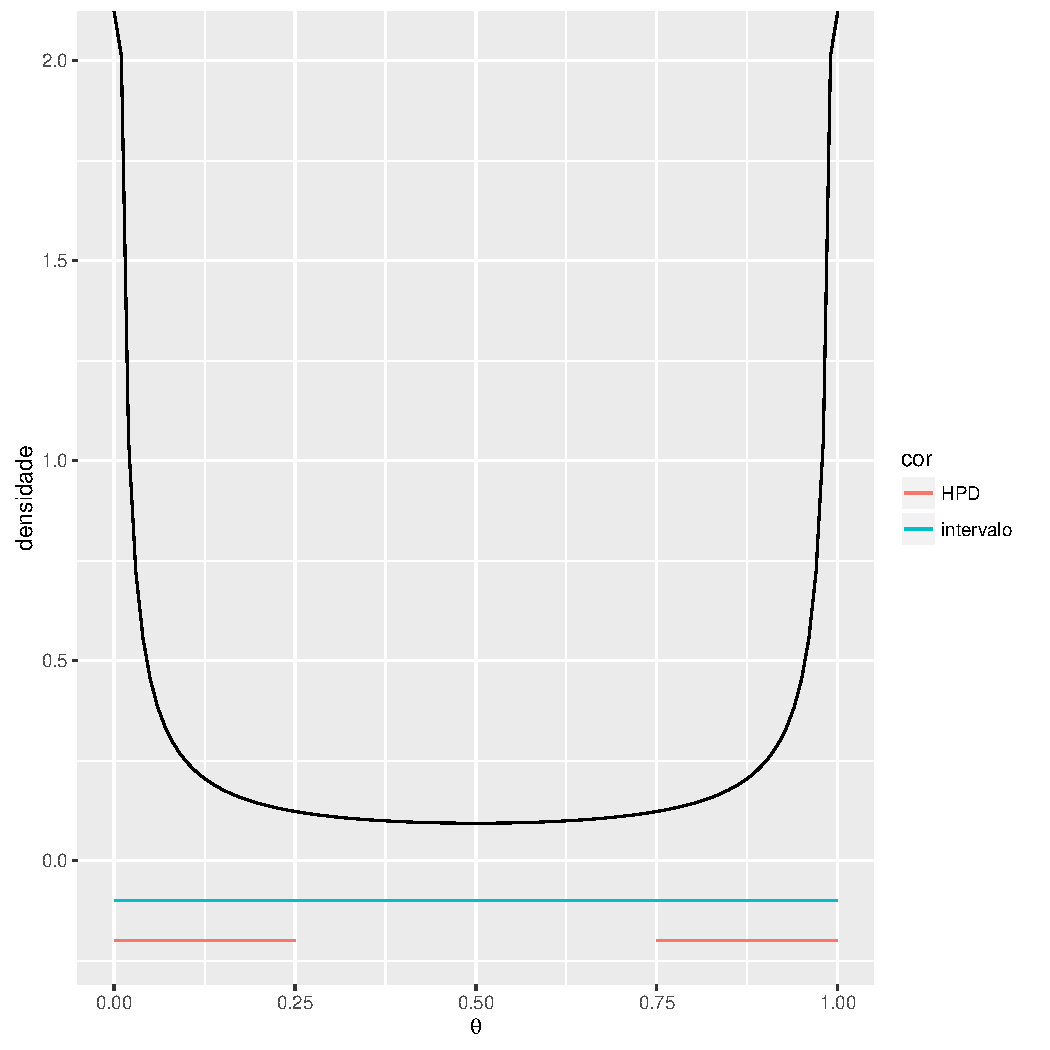
\includegraphics[scale=0.5]{chapter-decisions-bimodal-beta.pdf}
   \caption{Densidade da Beta$(0.05,0.05)$
   acompanhada de um intervalo de credibilidade 
   e o HPD.}
   \label{figure:bimodal-beta}
  \end{figure}
	
  \item Usando o \cref{thm:credible_interval_2},
  um possível intervalo de credibilidade, $[a,b]$,
  é tal que $\P(\theta < a|X) = 2.5\%$ e 
  $\P(\theta > b|X) = 2.5\%$.
  Podemos usar a função $qbeta$ no $R$ para
  obter os percentis da Beta$(0.05,0.05)$.
  O $R$ indica que eles são $8.8e-27$ e $1$.
  Portanto, o intervalo de credibilidade é
  praticamente o intervalo $[0,1]$ inteiro.

  \item Note pela \cref{figure:bimodal-beta} que 
  as regiões de maior densidade são
  os valores extremos à esquerda e à direita.
  Portanto, o HPD é composto por estes extremos.
  Como a distribuição a posteriori é simétrica em 
  torno de $0.5$,
  O HPD pode ser obtido determinando 
  $\P(\theta < a|X) = 47.5\%$ e
  $\P(\theta > b|X) = 52.5\%$.
  O HPD será $[0,a] \cup [b,1]$.
  Usando o $R$ encontramos que 
  $a \approx 0.25$ e $b \approx 0.75$.
 \end{enumerate}
}{}

\begin{exercise}[Sugestão de Aline Tonon]
 Considere o problema de determinar um intervalo de credibilidade, $(a,b)$, com a função de utilidade, $U((a,b),\theta)=\frac{\I(\theta \in (a,b))}{b-a}$. Prove que, se $(a^*,b^*)$ é um intervalo de credibilidade ótimo, então $f_{\theta|X}(a^*|X)=f_{\theta|X}(b^*|X)$.
\end{exercise}

\solution{\textbf{Solução}: Defina
 \begin{align*}
  g(a,b) := \E\left[U((a,b),\theta)|X\right]
  &= \E\left[\frac{\I(\theta \in (a,b))}{b-a}\bigg|X\right]
  = \frac{F_{\theta|X}(b|X)-F_{\theta|X}(a|X)}{b-a}
 \end{align*}
 Para que um ponto $(a,b)$ maximize $g(a,b)$,
 ele deve ser tal que $\nabla g(a,b)=\textbf{0}$.
 Note que
 \begin{align*}
  \nabla g(a,b) &= \left(\frac{\partial \frac{F_{\theta|X}(b|X)-F_{\theta|X}(a|X)}{b-a}}{\partial a}, \frac{\partial \frac{F_{\theta|X}(b|X)-F_{\theta|X}(a|X)}{b-a}}{\partial b}\right) \\
  &= \left(-\frac{f_{\theta|X}(a|X)(b-a)+(F_{\theta|X}(b|X)-F_{\theta|X}(a|X))}{(b-a)^2}, \frac{f_{\theta|X}(b|X)(b-a)-(F_{\theta|X}(b|X)-F_{\theta|X}(a|X))}{(b-a)^2} \right)
 \end{align*}
 Portanto, para que $\nabla g(a,b) = \textbf{0}$,
 obtemos
 \begin{align*}
  \begin{cases}
   f_{\theta|X}(a|X) = \frac{F_{\theta|X}(b|X)-F_{\theta|X}(a|X)}{b-a} \\
   f_{\theta|X}(b|X) = \frac{F_{\theta|X}(b|X)-F_{\theta|X}(a|X)}{b-a}
  \end{cases}
 \end{align*}
 Conclua que, se $(a^*,b^*)$ maximiza 
 a utilidade esperada, então
 $f_{\theta|X}(a^*|X)=f_{\theta|X}(b^*|X)$.
}{}

\begin{exercise}
 Considere o problema de determinar um intervalo de credibilidade, $(a,b)$, com a função de utilidade, $U((a,b),\theta)=\frac{k-(a-\theta)_{+}-(b-\theta)_{+}}{b-a}$. Prove que, se $(a^*,b^*)$ é um intervalo de credibilidade ótimo, então
 $F_{\theta|X}(a^*|X)=1-F_{\theta|X}(b^*|X)$.
\end{exercise}

\solution{\textbf{Solução}: Defina
 \begin{align*}
  g(a,b) := \E\left[U((a,b),\theta)|X\right]
  &= \E\left[\frac{k-(a-\theta)_{+}-(b-\theta)_{+}}{b-a}\bigg|X\right] \\
  &= \frac{k-\int_{-\infty}^{a}{(a-\theta)f_{\theta|X}(t|X)dt} -\int_{b}^{\infty}{(\theta-b)f_{\theta|X}(t|X)dt}}{b-a}
 \end{align*}
 Defina $h(a,b) := k-\int_{-\infty}^{a}{(a-\theta)f_{\theta|X}(t|X)dt} -\int_{b}^{\infty}{(\theta-b)f_{\theta|X}(t|X)dt}$.
 Para que um ponto $(a,b)$ maximize $g(a,b)$,
 ele deve ser tal que $\nabla g(a,b)=\textbf{0}$.
 Note que
 \begin{align*}
  \nabla g(a,b) &= \left(\frac{\partial g(a,b)}{\partial a}, \frac{\partial g(a,b)}{\partial b}\right) \\
  &= \left(\frac{-(b-a)\int_{-\infty}^{a}{f_{\theta|X}(t|X)dt} + h(a,b)}{(b-a)^2}, \frac{(b-a)\int_{b}^{\infty}{f_{\theta|X}(t|X)dt}-h(a,b)}{(b-a)^2} \right)
 \end{align*}
 Portanto, para que $\nabla g(a,b) = \textbf{0}$,
 é necessário que
 \begin{align*}
  \begin{cases}
   \int_{\infty}^{a}{f_{\theta|X}(t|X)dt} = 
   \frac{h(a,b)}{b-a}\\
   \int_{b}^{\infty}{f_{\theta|X}(t|X)dt} = 
   \frac{h(a,b)}{b-a}
  \end{cases}
 \end{align*}
 Conclua que, se $(a^*,b^*)$ maximiza a
 utilidade esperada, então
 $\int_{\infty}^{a^*}{f_{\theta|X}(t|X)dt}=\int_{b^*}^{\infty}{f_{\theta|X}(t|X)dt}$,
 isto é, 
 $F_{\theta|X}(a^*|X)=1-F_{\theta|X}(b^*|X)$.
}{}

